%
% rotation.tex
%
% (c) 2018 Prof Dr Andreas Müller, Hochschule Rapperswil
%
\documentclass[tikz]{standalone}
\usepackage{times}
\usepackage{txfonts}
\usepackage[utf8]{inputenc}
\usepackage{graphics}
\usepackage{ifthen}
\usepackage{color}
\usetikzlibrary{arrows,intersections}
\begin{document}

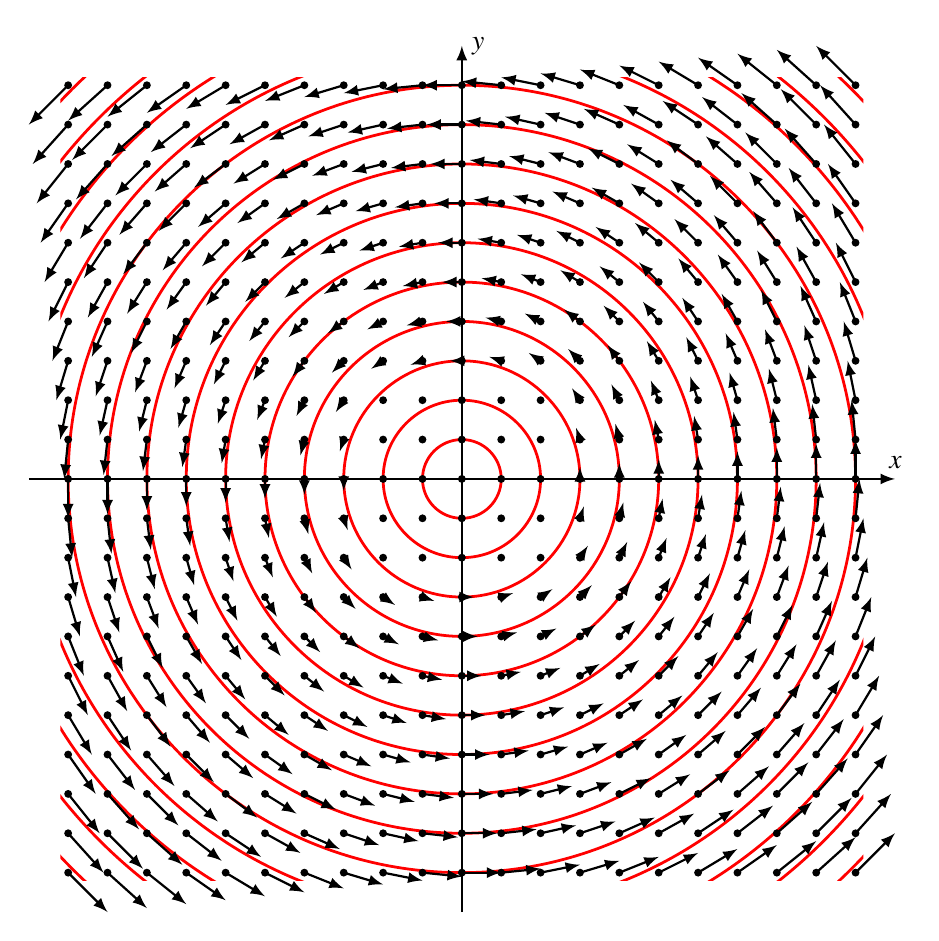
\begin{tikzpicture}[thick, >= latex]

\draw[->] (-5.5,0)--(5.5,0) coordinate[label={above:$x$}];
\draw[->] (0,-5.5)--(0,5.5) coordinate[label={right:$y$}];

\begin{scope}
\clip (-5.1,-5.1) rectangle (5.1,5.1);
\foreach \r in {0.5,1,...,9}{
	\draw[color=red,line width=1pt] (0,0) circle[radius={\r}];
}
\end{scope}

\def\a{0.1}

\foreach \x in {-5,-4.5,...,5}{
	\foreach \y in {-5,-4.5,...,5}{
		\fill ({\x},{\y}) circle[radius=0.05];
		\pgfmathparse{(((\x*\x+\y*\y) > 2) ? 1 : 0}
		\ifthenelse{1 = \pgfmathresult}{
			\draw[->] ({\x},{\y})--({\x-\a*\y},{\y+\a*\x});
		}{}
	}
}

\end{tikzpicture}
\end{document}

